
CMake是用C++编写的跨平台开源软件,可以自行编译它,但不推荐这样做。可以从官方网页下载预编译的二进制文件,网址是\url{https://cmake.org/download/}。

基于Unix的系统可以直接使用命令行进行安装。

\begin{tcolorbox}[colback=blue!5!white,colframe=blue!75!black,title=Note]
CMake并不附带编译器。若系统中还没有安装编译器,需要在使用CMake之前安装或提供它们的路径。确保将可执行文件的路径添加到PATH环境变量中,以便CMake能够找到它们。

为了避免在阅读本书时遇到的工具和依赖问题,建议使用Docker。
\end{tcolorbox}

来了解一下可以使用CMake的环境。

\subsubsubsection{1.3.1\hspace{0.2cm}Docker}

Docker (\url{https://www.docker.com/})是一个跨平台工具,提供操作系统级虚拟化,允许应用程序以完整(称为容器)的形式发布。这些是捆绑包,包含软件及其运行所需的所有库、依赖项和工具。Docker可在隔离的轻量级环境中运行容器。

这个概念使得共享工具链非常方便,这些工具链是必需的,并且是配置好的。

Docker平台有一个镜像的公共存储库\url{https://registry.hub.docker.com/},提供了数百万个现成的镜像。

方便起见,我发布了两个Docker镜像:

\begin{itemize}
\item 
swidzinski/cmake:toolchain: 包含了使用CMake构建所必需的策划工具和依赖项。

\item 
swidzinski/cmake:examples: 包含了前面的工具链,以及本书中的所有项目和示例。
\end{itemize}

第一个选项是为那些只想要一个干净镜像的读者;第二个选项可以在阅读本章时,使用示例进行实践。

可以按照Docker官方文档的说明安装Docker(请参考\url{docs.docker.com/get-docker})。然后,在终端中执行以下命令下载镜像并启动容器:

\begin{tcblisting}{commandshell={}}
$ docker pull swidzinski/cmake:examples
$ docker run -it swidzinski/cmake:examples
root@b55e271a85b2:root@b55e271a85b2:#
\end{tcblisting}

注意,所有的例子都在这样格式的目录中:\texttt{/root/examples/examples/chapter-<n>/<m>-<title>}。

\subsubsubsection{1.3.2\hspace{0.2cm}Windows}

Windows上安装很简单——只需下载32位或64位的版本,可以为Windows安装程序选择便携ZIP或MSI包。

对于ZIP包,必须将CMake的bin目录添加到PATH环境变量中,这样就可以在目录中使用CMake:

\begin{tcblisting}{commandshell={}}
'cmake' is not recognized as an internal or external command,
operable program or batch file.
\end{tcblisting}

若更喜欢简单的方式,就使用MSI安装:

\begin{center}
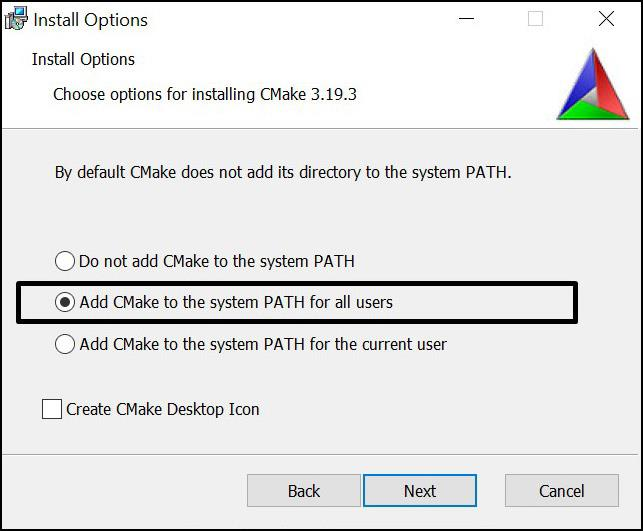
\includegraphics[width=0.6\textwidth]{content/1/chapter1/images/2.jpg}\\
图1.2 安装向导可以设置PATH环境变量
\end{center}

这是一个开源软件,所以可以自己构建CMake。首先,必须在系统上获得CMake的二进制副本。那么,若有自己的构建工具,为什么还要使用其他构建工具呢?CMake的代码贡献者可以使用此方式生成新版本的CMake。

在Windows上,还需要一个构建工具来完成由CMake启动的构建过程。这里的选择是Visual Studio,社区版可以从微软的网站上免费获得:\url{https://visualstudio.microsoft.com/downloads/}。

\subsubsubsection{1.3.3\hspace{0.2cm}Linux}

Linux上获得CMake与获得其他包一样,只需在终端使用包管理器即可。软件包的版本不保证是最新,若想要最新版本,可以下载安装脚本:

\hspace*{\fill} \\ %插入空行
\noindent
\textbf{Linux x86\_64的安装脚本}

\begin{tcblisting}{commandshell={}}
$ wget -O - https://github.com/Kitware/CMake/releases/download/
v3.20.0/cmake-3.20.0-linux-x86_64.sh | bash
\end{tcblisting}

\hspace*{\fill} \\ %插入空行
\noindent
\textbf{Linux aarch64的安装脚本}

\begin{tcblisting}{commandshell={}}
$ wget -O - https://github.com/Kitware/CMake/releases/download/
v3.20.0/cmake-3.20.0-Linux-aarch64.sh | bash
\end{tcblisting}

\hspace*{\fill} \\ %插入空行
\noindent
\textbf{Debian/Ubuntu的安装包}

\begin{tcblisting}{commandshell={}}
$ sudo apt-get install cmake
\end{tcblisting}

\hspace*{\fill} \\ %插入空行
\noindent
\textbf{Red Hat的安装包}

\begin{tcblisting}{commandshell={}}
$ yum install cmake
\end{tcblisting}

\subsubsubsection{1.3.4\hspace{0.2cm}macOS}

这个平台也得到了CMake开发人员的大力支持。可以通过MacPorts安装:

\begin{tcblisting}{commandshell={}}
$ sudo port install cmake
\end{tcblisting}

或者,使用Homebrew:

\begin{tcblisting}{commandshell={}}
$ brew install cmake
\end{tcblisting}

\subsubsubsection{1.3.5\hspace{0.2cm}使用源码构建}

若以上方法都失败了——或者是在特殊的平台上——可以从官方网站下载源代码,自行编译:

\begin{tcblisting}{commandshell={}}
$ wget https://github.com/Kitware/CMake/releases/download/
v3.20.0/cmake-3.20.0.tar.gz
$ tar xzf cmake-3.20.0.tar.gz
$ cd cmake-3.20.0
$ ./bootstrap
$ make
$ make install
\end{tcblisting}

从源码构建相对较慢,需要更多步骤。但通过这种方式,可以保证使用最新版本的CMake。与Linux可用的包相比,这一点尤其明显:系统版本越老,得到的更新就越少。

我们已经安装了CMake,现在来了解如何使用它吧!









